%&latex

%%%%%%%%%%%%%%%%%%%%%%%%%%%%%%%%%%
%				TeX Configuration
%%%%%%%%%%%%%%%%%%%%%%%%%%%%%%%%%%

%%%\documentclass[9pt,blockstyle,nonatbib]{sigplanconf}
%%%%\documentclass[11pt,times,letterpaper]{article}
%%%
%%%%\usepackage[top=.75in,left=.75in,right=.75in,bottom=.75in]{geometry}
%%%
%%%\usepackage{times} % For times font
%%%\usepackage{graphics}
%%%\usepackage[usenames]{color}
%%%\usepackage{color,graphicx}  % To import color graphics
%%%\usepackage{latexsym,amssymb,epsf}
%%%\usepackage{setspace}  % For single/double spacing
%%%\usepackage{subfigure} % subfigure support
%%%\usepackage{tabularx} % For tabular in author 
%%%\usepackage{multirow}
%%%\usepackage{booktabs}
%%%\usepackage{paralist} % For tabular in author 
%%%%\usepackage{titling} % For complicated author list layout
%%%\usepackage{cite} % To sort citation numbers
%%%\usepackage[format=hang,indention=-0.5in,margin=10pt,font={small,sf},labelfont=bf]{caption}  %Get figure captions to look sensible
%%%\usepackage{amsfonts}
%%%\usepackage{xspace} 
%%%\usepackage{fancyhdr}
%%%%\usepackage[numbers,square,sort]{natbib} 
%%%
%%%
%%%%\usepackage{url}
%%%%\usepackage{epsf}
%%%%\usepackage{pslatex}
%%%%\usepackage{amssymb}
%%%%\usepackage{enumerate}
%%%%\usepackage{algorithm}
%%%%\usepackage{colordvi}
%%%%\usepackage{floatflt}


\newcommand{\fix}{ {\bf \textcolor{red}{FIXME} }}
%\newcommand{\fixme}[1]{\textbf{\textcolor{red}{[ Fixme: #1]}}}


\newcommand{\PowerRouting}{Power Routing\xspace}

\newcommand{\MACClong}{Scientific Computing Data Center}
\newcommand{\MACC}{SCDC}

\newcommand{\field}[1]{\mathbb{#1}}


\newenvironment{packed_itemize}{
\begin{itemize}
  \setlength{\topsep}{0pt}
  \setlength{\partopsep}{0pt}
  \setlength{\itemsep}{0pt}
  \setlength{\parskip}{0pt}
  \setlength{\parsep}{0pt}
}{\end{itemize}}
%%%
%%%\widowpenalty=10000
%%%\clubpenalty=10000
%%%\raggedbottom
%%%
%%%% Shrink bib font 
%%%\def \bibfont {\normalsize}
%%%
%%%%\pagenumbering{arabic}

% authors for Appendix
{
\centering
Steven Pelley, David Meisner, Pooya Zandevakili, \\
Thomas F. Wenisch, and Jack Underwood \\
\vspace{2\baselineskip}
}

%	Abstract

%\singlespacing
%\vspace{-0.7in}
%\begin{abstract}
%\small
\emph{Data center power infrastructure incurs massive capital costs, which typically exceed energy costs over the life of the facility. To squeeze maximum value from the infrastructure, researchers have proposed over-subscribing power circuits, relying on the observation that peak loads are rare.  To ensure availability, these proposals employ} power capping, \emph{which throttles server performance during utilization spikes to enforce safe power budgets.  However, because budgets must be enforced locally---at each power distribution unit (PDU)---local utilization spikes may force throttling even when power delivery capacity is available elsewhere.  Moreover, the need to maintain reserve capacity for fault tolerance on power delivery paths magnifies the impact of utilization spikes.}

\emph{In this paper, we develop mechanisms to better utilize installed power infrastructure, reducing reserve capacity margins and avoiding performance throttling. Unlike conventional high-availability data centers, where collocated servers share identical primary and secondary power feeds, we reorganize power feeds to create} shuffled \emph{power distribution topologies. Shuffled topologies spread secondary power feeds over numerous PDUs, reducing reserve capacity requirements to tolerate a single PDU failure.  Second, we propose} Power Routing, \emph{which schedules IT load dynamically across redundant power feeds to: (1) shift slack to servers with growing power demands, and (2) balance power draw across AC phases to reduce heating and improve electrical stability.  We describe efficient heuristics for scheduling servers to PDUs (an NP-complete problem). Using data collected from nearly 1000 servers in three production facilities, we demonstrate that these mechanisms can reduce the required power infrastructure capacity relative to conventional high-availability data centers by 32\% without performance degradation.}

%%%\end{abstract}
%%%
%%%\normalsize
%%%
%%%\category{C.5.5}{Computer System Implementation}{Servers}
%%%
%%%\terms
%%%Design, Measurement
%%%
%%%\keywords
%%%power infrastructure, data centers



%	Introduction
\section{Introduction}

Data center power consumption continues to grow at an alarming pace; it is projected to reach 100 billion kWh at an annual cost of \$7.4 billion within two years \cite{EPA07}, with a world-wide carbon-emissions impact similar to that of the entire Czech Republic \cite{Mankoff08}. In light of this trend, computer systems researchers, application designers, power and cooling engineers, and governmental bodies have all launched research efforts to improve data center energy efficiency.  These myriad efforts span numerous aspects of data center design (server architecture \cite{Lefurgy03,Meisner09}, scheduling \cite{Moore06, Parolini08},  power delivery systems \cite{Fan07}, cooling infrastructure \cite{Patel02}, etc.).  However, with few exceptions, existing efforts focus narrowly on energy-efficiency of single subsystems, without considering global interactions or implications across data center subsystems. 

As sophisticated power management features proliferate, the dynamic range of data center power draw (as a function of utilization) is increasing, and interactions among power management strategies across subsystems grow more complex; subsystems can no longer be analyzed in isolation.   Even questions that appear simple on their face can become quite complicated.

Reasoning about total data center power is difficult because of the diversity and complexity of data center infrastructure.  Five distinct sub-systems (designed and marketed by different industry segments) account for most of a data center's power draw:  (1) servers and storage systems, (2) power conditioning equipment, (3) cooling and humidification systems, (4) networking equipment, and (5) lighting/physical security.  Numerous sources have reported power breakdowns \cite{EPA07,Meisner09}; Table~\ref{table::PowerDistribution} illustrates a typical breakdown today.   The first three subsystems dominate and their power draw can vary drastically with data center utilization. Cooling power further depends on ambient weather conditions around the data center facility. Even the distribution of load in each subsystem can affect power draws, as the interactions among sub-systems are non-linear
%(e.g., thermal hot spots disproportionately increase cooling requirements).

In this paper, our objective is to provide tools to the computer systems community to assess and reason about total data center power.  Our approach is two-fold, targeting both \emph{data center simulation} and \emph{abstract analytic modeling}.  First, we have collected a set of detailed power models (from academic sources, industrial white papers, and product data sheets) for each critical component of data center infrastructure, which describe power draw as a function of environmental and load parameters.  Each model describes the power characteristics of a single device (i.e., one server or computer room air handler (CRAH)) and, as such, is suitable for integration into a detailed data center simulator.  We describe how these models interact (i.e., how utilization, power, and heat flow among components) and outline the design of such a simulator. To our knowledge, we are the first to describe an integrated data center simulation infrastructure; its implementation is underway.

Although these detailed models enable data center simulation, they do not allow direct analytic reasoning about total data center power.  Individual components' power draw vary non-linearly with localized conditions (i.e., temperature at a CRAH inlet, utilization of an individual server), that require detailed simulation to assess precisely.  Hence, to enable back-of-the-envelope reasoning, we develop an \emph{abstract model} that replaces key steps of the data center simulation process with simple parametric models that enable analysis of average behavior.  In particular, we abstract away time-varying scheduling/load distribution across servers and detailed tracking of the thermodynamics of data center airflow.  Our abstract model provides insight into how data center sub-systems interact and allows quick comparison of energy-efficiency optimizations.

\begin{table}[t]
\begin{center}
\caption{ \textbf{Typical Data Center Power Breakdown.} }
\label{table::PowerDistribution}

\begin{tabularx}{\linewidth}{c c c c c}
    \toprule
    Servers & Cooling & Power Cond. & Network & Lighting \\
    \midrule
    56\% & 30\% & 8\% & 5\% & 1\% \\
    \bottomrule
  \end{tabularx}
\end{center}

\end{table}


% Background
\section{Background}
\label{section::background}

We begin with a brief overview of data center power provisioning infrastructure and power capping mechanisms.  A more extensive introduction to these topics is available in \cite{BarrosoBook09}.

\begin{figure*}[t]
\centering
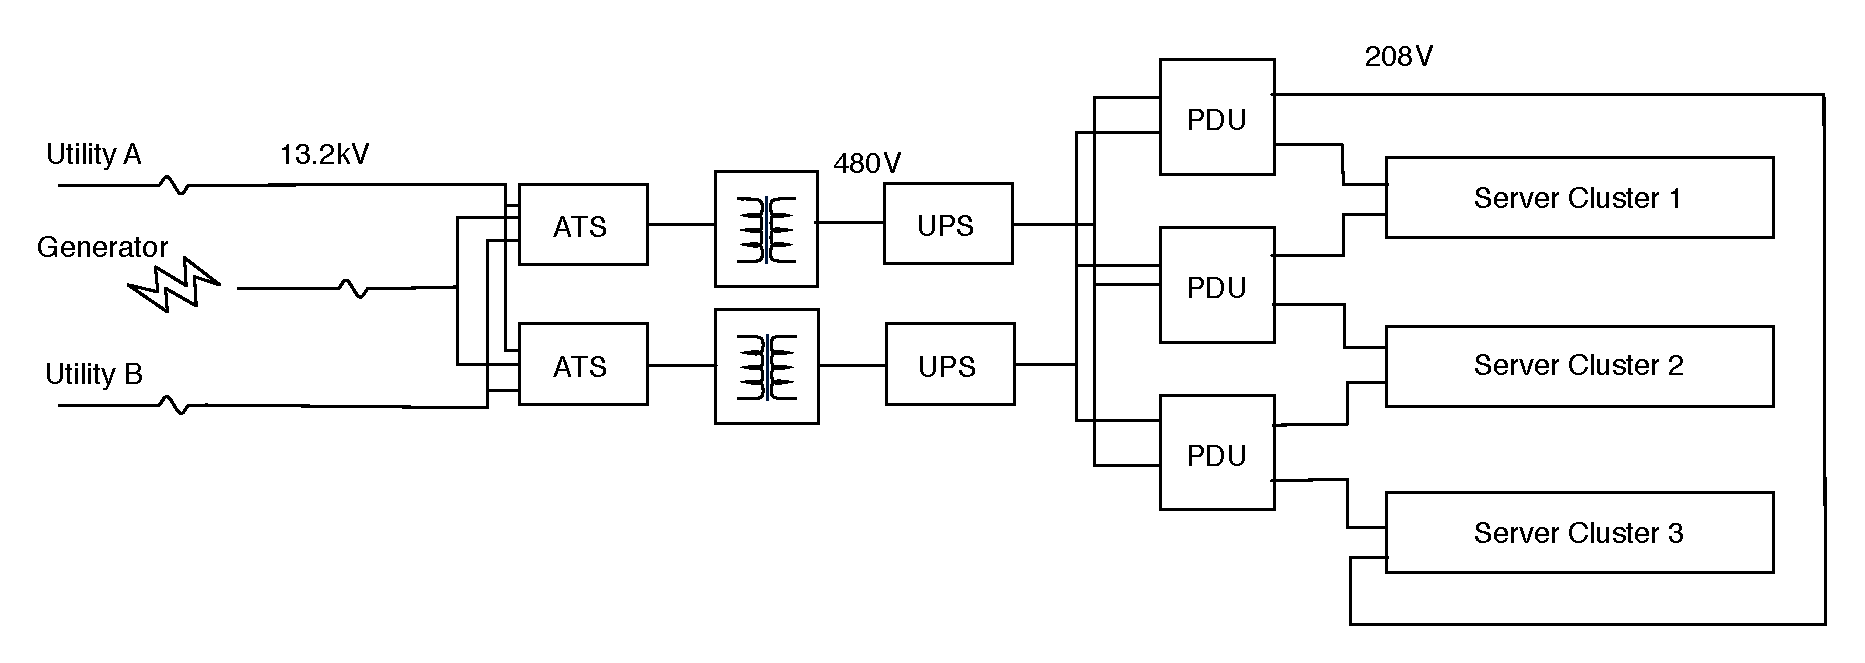
\includegraphics[scale=.5]{Appendices/PowerRouting/figure/redundant.eps}
\vspace{-0.15 in}
\caption{ \textbf{Example power delivery system for a high-availability data center.} }
\vspace{-0.15 in}
\label{figure::redundant}
\end{figure*}


\textbf{Conventional power provisioning.} Today, most data centers operate according to power provisioning policies that assure sufficient capacity for every server. These policies are enforced by the data center operators at system installation time, by prohibiting deployment of any machine that creates the potential for overload.  Operators do their best to estimate systems' peak power draws, either through stress-testing, from vendor-supplied calculators, or through de-rating of nameplate specifications.

In high-availability data centers, power distribution schemes must also provision redundancy for fault tolerance; system deployments are further restricted by these redundancy requirements.  The Uptime Institute classifies data centers into tiers based on the nature and objectives of their infrastructure redundancy \cite{Turner05}. Some data centers provide no fault tolerance (Tier-1), or provision redundancy only within major power infrastructure components, such as the UPS system (Tier-2).  Such redundancy allows some maintenance of infrastructure components during operation, and protects against certain kinds of faults, but numerous single points-of-failure remain.  Higher-tier data centers provide redundant power delivery paths to each server. \PowerRouting is targeted at these data centers, as it exploits the redundant delivery paths to shift power delivery capacity.

\textbf{Example: A high-availability power system.} Figure~\ref{figure::redundant} illustrates an example of a high-availability power system design and layout for a data center with redundant distribution paths.  The design depicted here is based on the power architecture of the Michigan Academic Computer Center (MACC), the largest (10,000 square feet; 288 racks; 4MW peak load including physical infrastructure) of the three facilities providing utilization traces for this study. Utility power from two substations and a backup generator enter the facility at high voltage (13.2 kVAC) and meet at redundant automated transfer switches (ATS) that select among these power feeds.  These components are sized for the peak facility load (4MW), including all power infrastructure and cooling system losses.  The ATS outputs in turn are transformed to a medium voltage (480 VAC) and feed redundant uninterruptible power supply (UPS) systems, which are also each sized to support the entire facility.  These in turn provide redundant feeds to an array of power distribution units (PDUs) which further transform power to 208V 3-phase AC.  

PDUs are arranged throughout the data center such that each connects to two neighboring system clusters and each cluster receives redundant power feeds from its two neighboring PDUs.  The power assignments wrap from the last cluster to the first.  We refer to this PDU arrangement as a \emph{wrapped topology}. The wrapped topology provides redundant delivery paths with minimal wiring and requires each PDU to be sized to support  at most 150\% of the load of its connected clusters, with only a single excess PDU beyond the minimum required to support the load (called an ``N+1" configuration).  In the event of any PDU fault, 50\% of its supported load fails over to each of its two neighbors.  PDUs each support only a fraction of the data center's load, and can range in capacity from under ten to several hundred kilowatts.

Power is provided to individual servers through connectors (called ``whips"), that split the three phases of the 208VAC PDU output into the 120VAC single-phase circuits familiar from residential wiring.  (Some equipment may operate at higher voltages or according to other international power standards.) Many modern servers include redundant power supplies, and provide two power cords that can be plugged into whips from each PDU.  In such systems, the server internally switches or splits its load among its two power feeds.  For servers that provide only a single power cord, a rack-level transfer switch can connect the single cord to redundant feeds.

The capital costs of the power delivery infrastructure are concentrated at the large, high-voltage components: PDUs, UPSs, facility-level switches, generators, transformers and the utility feed.  The rack-level components cost a few thousand dollars per rack (on the order of \$1 per provisioned Watt), while the facility-level components can cost \$10-\$25 per provisioned Watt \cite{BarrosoBook09,Turner06}, especially in facilities with such high levels of redundancy.  With \PowerRouting, we focus on reducing the required provisioning of the facility-scale components while assuring a balanced load over the PDUs.  Though circuit breakers typically limit current both at the PDU's breaker panels and on the individual circuits in each whip, it is comparatively inexpensive to provision these statically to avoid overloads.  Though \PowerRouting is applicable to manage current limits on individual circuits, we focus on enforcing limits at the PDU level in this work.

\textbf{Phase balance}. In addition to enforcing current limits and redundancy, it is also desirable for a power provisioning scheme to balance power draw across the three phases of AC power supplied by each PDU.  Large phase imbalances can lead to current spikes on the neutral wire of a 3-phase power bus, voltage and current distortions on the individual phases, and generally increase heat dissipation and reduce equipment lifetime \cite{Gruzs90}.  Data center operators typically manually balance power draw across phases by using care in connecting equipment to particular receptacles wired to each phase.  \PowerRouting can automatically enforce phase balance by including it as explicit constraints in its scheduling algorithm. 


\textbf{Power capping.} Conservative, worst-case design invariably leads to power infrastructure over-provisioning \cite{Govindan09,Ranganathan06,Fan07,Wang09}.  Power capping mechanisms allow data center operators to sacrifice some performance in rare utilization spikes in exchange for substantial cost savings in the delivery infrastructure, without the risk of cascading failures due to an overload. In these schemes, some centralized control mechanism establishes a power budget for each server (e.g., based on historical predictions or observed load in the previous time epoch).  An actuation mechanism then enforces these budgets.  

\begin{figure*}[t]
\centering
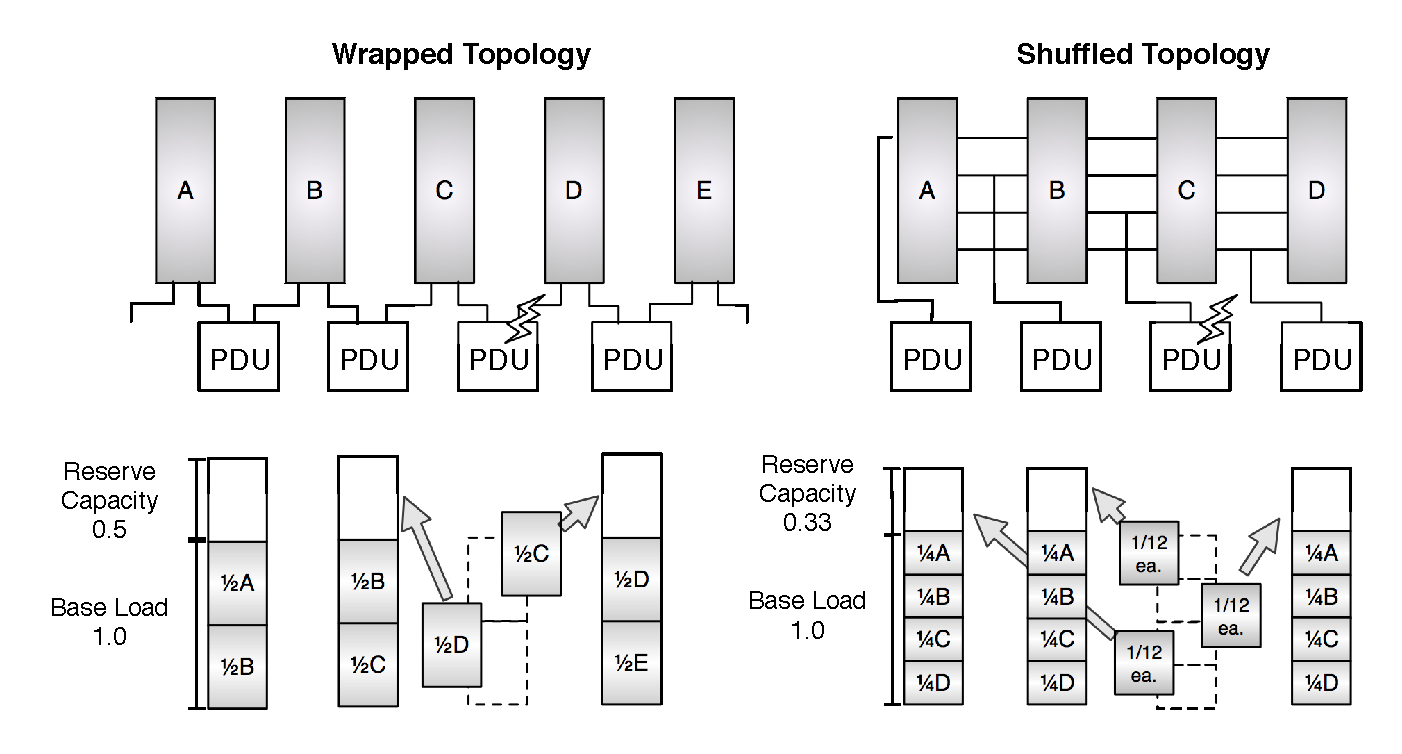
\includegraphics[width = 6.0 in]{Appendices/PowerRouting/figure/failover2.eps}
\caption{ \textbf{Reduced reserve capacity under shuffled topologies (4 PDUs, fully-connected topology).}}
\label{figure::failover}
\vspace{-.1 in}
\end{figure*}

The most common method of enforcing power budgets is through control loops that sense actual power draw and modulate processor frequency and voltage to remain within budget.  Commercial systems from IBM \cite{Popa06} and HP \cite{HP09} can enforce budgets to sub-watt granularities at milli-second timescales.  Researchers have extended these control mechanisms to enforce caps over multi-server chassis, larger ensembles, and entire clusters \cite{Ranganathan06,Lefurgy08,Wang08, Femal05}, examine optimal power allocation among heterogeneous servers \cite{Gandhi09b} and identify the control stability challenges when capping at multiple levels of the power distribution hierarchy \cite{Raghavendra08,Wang09}. Others have examined extending power management to virtualized environments \cite{Nathuji07}.  Soft fuses \cite{Govindan09} apply the notion of power budgets beyond the individual server and enforce sustained power budgets, which allow for transient overloads that the power infrastructure can support.  Finally, prior work considers alternative mechanisms for enforcing caps, such as modulating between active and sleep states \cite{Gandhi09a}. 

Like prior work, \PowerRouting relies on a power capping mechanism as a safety net to ensure extended overloads can not occur.  However, \PowerRouting is agnostic to how budgets are enforced. For simplicity, we assume capping based on dynamic frequency and voltage scaling, the dominant approach.  

Though rare, peak utilization spikes do occur in some facilities.  In particular, if a facility runs a single distributed workload balanced over all servers (e.g., as in a web search cluster), then the utilization of all servers will rise and fall together \cite{Fan07}.  No scheme that over-subscribes the physical infrastructure can avoid performance throttling for such systems. The business decision of whether throttling is acceptable in these rare circumstances is beyond the scope of this study; however, for any given physical infrastructure budget, \PowerRouting reduces performance throttling relative to existing capping schemes, by shifting loads among PDUs to locate and exploit spare capacity.



% Design
\section{Power Routing.}
\label{section::powerrouting}


\PowerRouting relies on two central concepts.  First, it exploits \emph{shuffled topologies} for power distribution to increase the connectivity between servers and diverse PDUs.  Shuffled topologies spread responsibility to sustain the load on a failing PDU, reducing the required reserve capacity per PDU.  Second, \PowerRouting relies on a \emph{scheduling} algorithm to assign servers' load across redundant distribution paths while balancing loads over PDUs and AC phases.  When loads are balanced, the provisioned capacity of major power infrastructure components (PDUs, UPSs, generators, and utility feeds) can be reduced, saving capital costs.  We first detail the design and advantages of shuffled topologies, and then discuss \PowerRouting.

\subsection{Shuffled Topologies.}
\label{section::intermixed}

\begin{figure*}[t]
\centering
\subfigure[Wrapped (conventional)]{
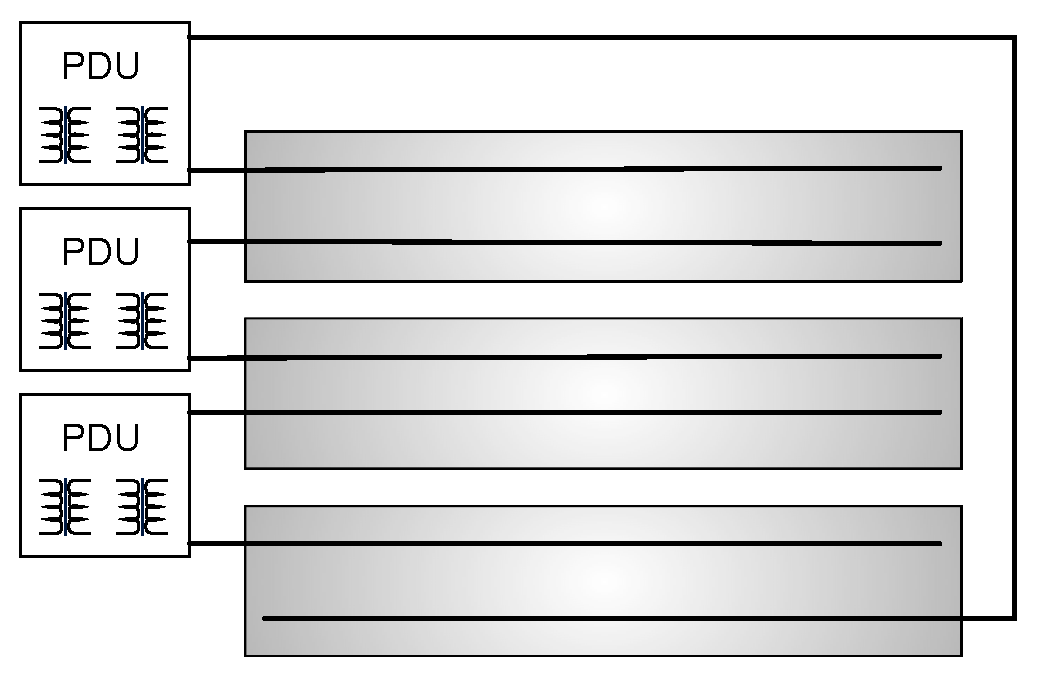
\includegraphics[scale=.3]{Appendices/PowerRouting/figure/standard3.eps}
\label{figure::wrapped}
}
\hspace{0.3in}
\subfigure[Fully-connected]{
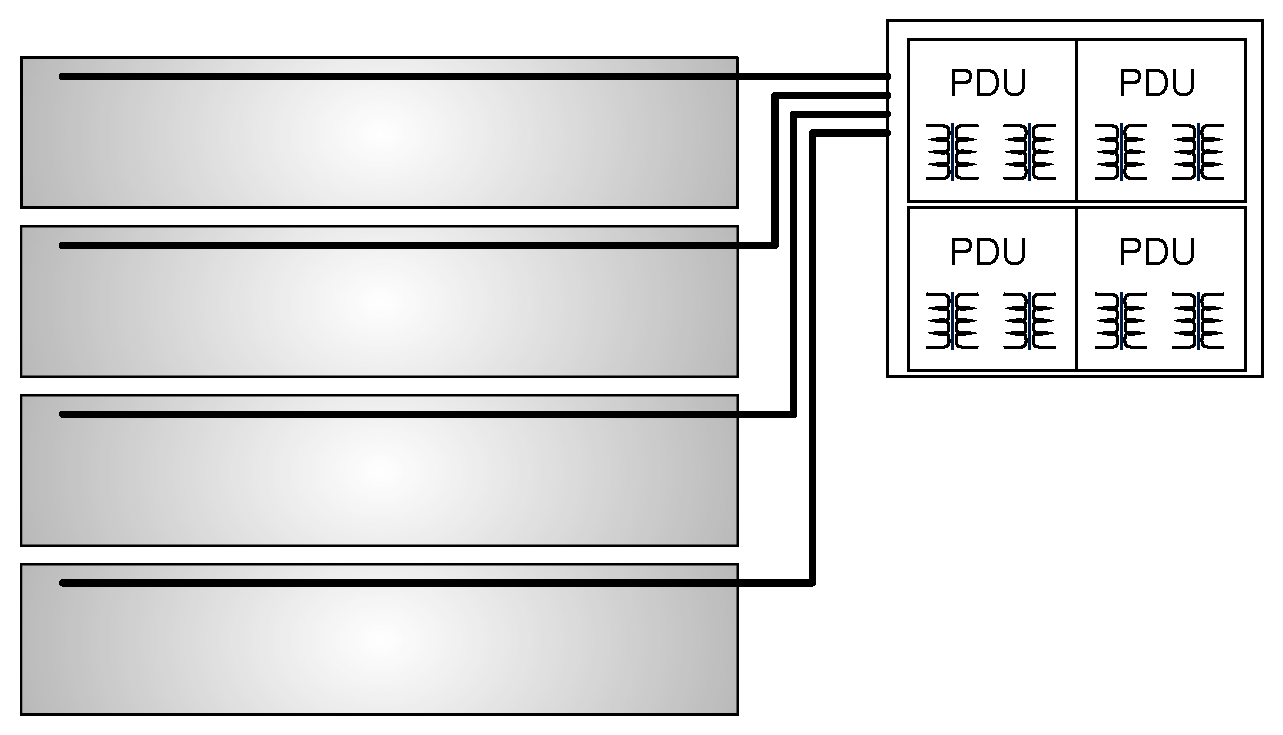
\includegraphics[scale=.3]{Appendices/PowerRouting/figure/full2.eps}
\label{figure::connected}
}
\qquad
\subfigure[Serpentine]{
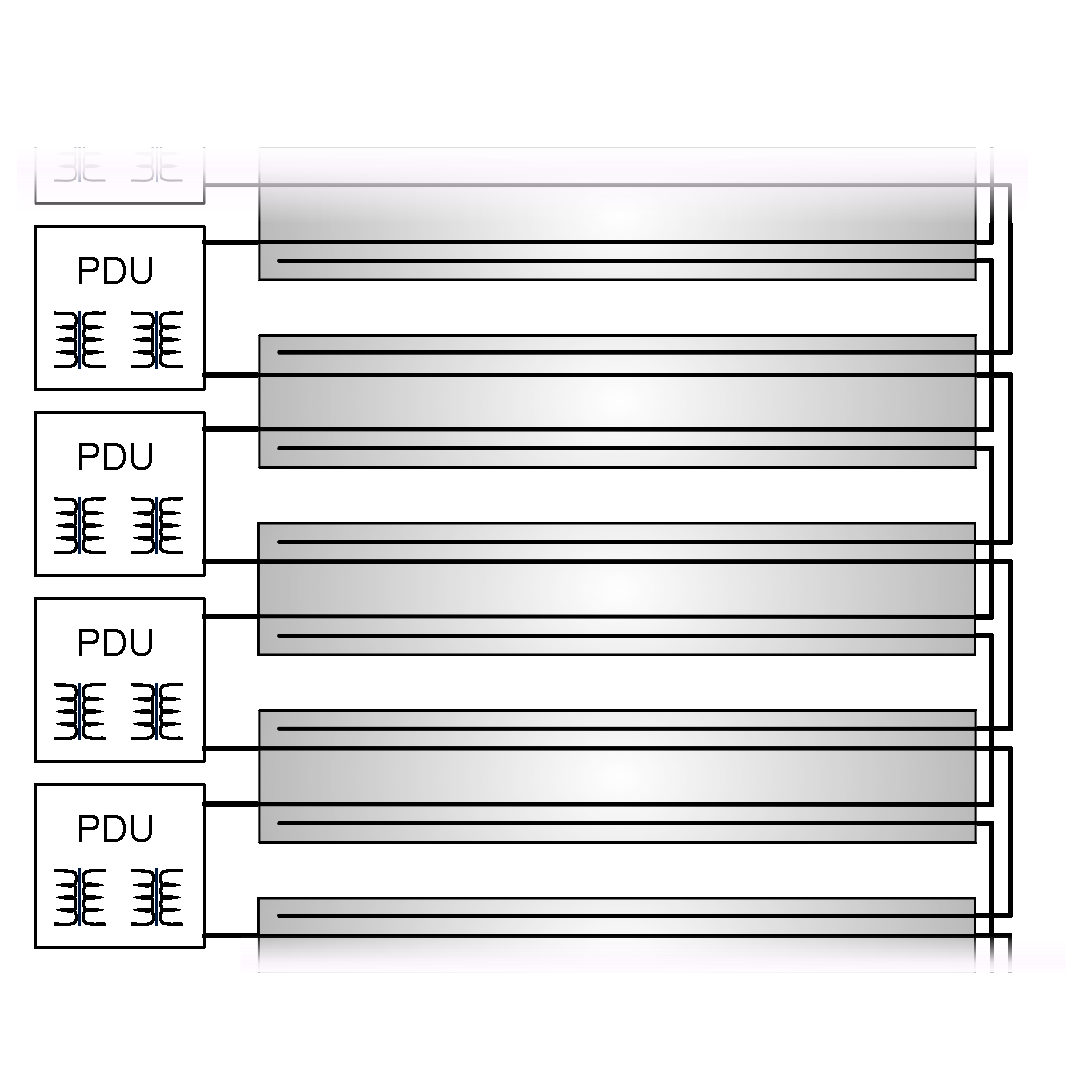
\includegraphics[scale=.3]{Appendices/PowerRouting/figure/ring.eps}
\label{figure::ring}
}
\hspace{0.5in}
\subfigure[X-Y]{
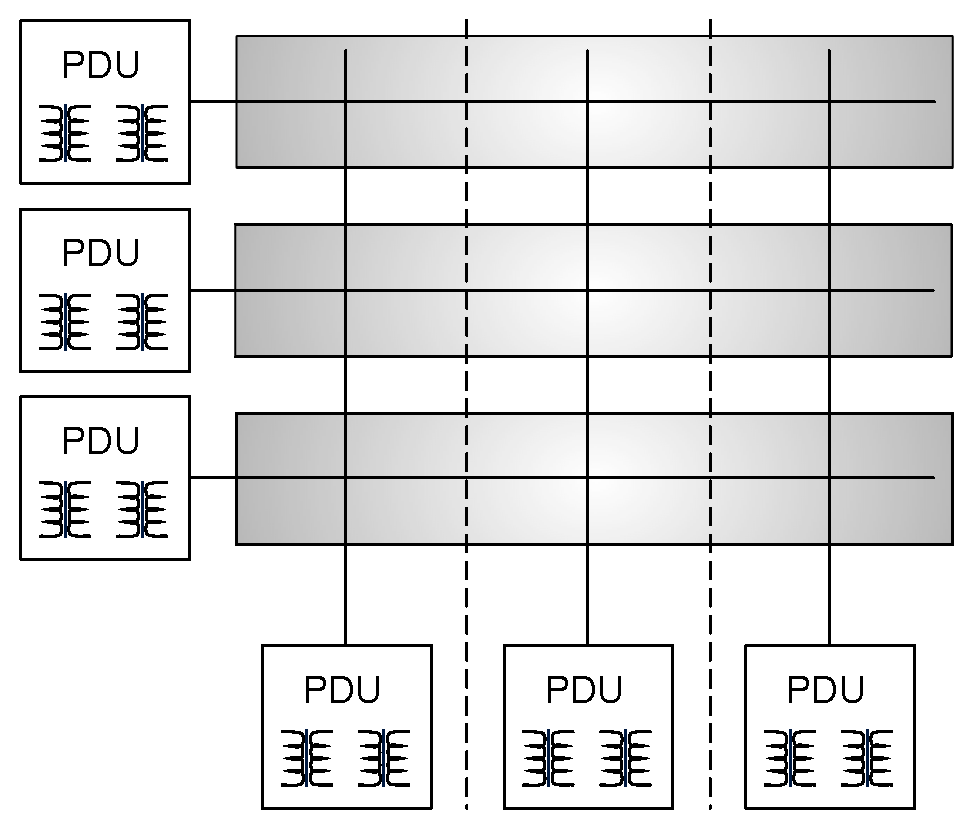
\includegraphics[scale=.3]{Appendices/PowerRouting/figure/xy3.eps}
\label{figure::xy}
}

\vspace{-0.10 in}
\caption{ \textbf{Shuffled power distribution topologies.} }
\vspace{-0.15 in}
\label{figure::topologies}
\end{figure*}

In high-availability data centers, servers are connected to two PDUs to ensure uninterrupted operation in the event of a PDU fault.  A naive (but not unusual) connection topology provisions paired PDUs for each cluster of machines.  Under this data center design, each PDU must be sized to support the full worst-case load of the entire cluster; hence, the power infrastructure is 50\% utilized in the best case. As described in Section~\ref{section::background}, the more sophisticated ``wrapped" topology shown in Figure~\ref{section::background} splits a failed PDU's load over two neighbors, allowing each PDU to be sized to support only 150\% of its nominal primary load.  

By spreading the responsibility for failover further, to additional PDUs, the spare capacity required of each PDU can be reduced---the more PDUs that cooperate to cover the load of a failed PDU, the less reserve capacity is required in the data center as a whole.  In effect, the reserve capacity in each PDU protects multiple loads (which is acceptable provided there is only a single failure). 

Figure~\ref{figure::failover} illustrates the differing reserve capacity requirements of the wrapped topology and a shuffled topology where responsibility for reserve capacity is spread over three PDUs.  The required level of reserve capacity at each PDU is approximately $X / N$, where $X$ represents the cluster power demand, and $N$ the number of PDUs cooperating to provide reserve capacity. (Actual reserve requirements may vary depending on the instantaneous load on each phase).

The savings from shuffled topologies do not require any intelligent switching capability; rather, they require only increased diversity in the distinct combinations of primary and secondary power feeds for each server (ideally covering all combinations equally).   

The layout of PDUs and power busses must be carefully considered to yield feasible shuffled wiring topologies.   Our distribution strategies rely on overhead power busses \cite{Rasmussen129} rather than conventional under-floor conduits to each rack.  The power busses make it easier (and less costly) to connect many, distant racks to a PDU.  Power from each nearby bus is routed to a panel at the top of each rack, and these in turn connect to vertical whips (i.e., outlet strips) that supply power to individual servers.  The whips provide outlets in pairs (or a single outlet with an internal transfer switch) to make it easy to connect servers while assuring an appropriate mix of distinct primary and secondary power feed combinations.

Though overhead power busses are expensive, they still account for a small fraction of the cost of large-scale data center power infrastructure.  Precise quantification of wiring costs is difficult without detailed facility-specific architecture and engineering. We neglect differences in wiring costs when estimating data center infrastructure costs, and instead examine the (far more significant) impact that topologies have on the capacity requirements of the high-voltage infrastructure.  The primary difficulty of complex wiring topologies lies in engineering the facility-specific geometry of the large (and dangerous) high-current overhead power rails; a challenge that we believe is surmountable.

We propose three shuffled power distribution topologies that improve on the wrapped topology of current high-availability data centers.  The \emph{fully connected} topology collocates all PDUs in one corner of the room, and routes power from all PDUs throughout the entire facility.  This topology is not scalable. However, we study it as it represents an upper bound on the benefits of shuffled topologies. We further propose two practical topologies.  The \emph{X-Y} topology divides the data center into a checkerboard pattern of power zones, routing power both north-south and east-west across the zones.  The \emph{serpentine} topology extends the concept of the wrapped topology (see Figure~\ref{figure::redundant}) to create overlap among neighboring PDUs separated by more than one row.

Each distribution topology constrains the set of power feed combinations available in each rack in a different manner.  These constraints in turn affect the set of choices available to the \PowerRouting scheduler, thereby impacting its effectiveness.  


\textbf{Wrapped Topology}.  Figure~\ref{figure::wrapped} illustrates the wrapped topology, which is our term for the conventional  high-availability data center topology (also seen in Figure~\ref{figure::redundant}).  This topology provides limited connectivity to PDUs, and is insufficient for \PowerRouting. 

\textbf{Fully-connected Topology}.  Figure~\ref{figure::connected} illustrates the fully-connected topology.  Under this topology, power is routed from every PDU to every rack. As noted above, the fully-connected topology does not scale and is impractical in all but the smallest data centers.  However, one scalable alternative is to organize the data center as disconnected islands of fully-connected PDUs and rack clusters.  Such a topology drastically limits \PowerRouting flexibility, but can scale to arbitrary-sized facilities.

\textbf{Serpentine Topology}.  Figure~\ref{figure::ring} illustrates the serpentine topology.  Under this topology, PDUs are located at one end of the data centers' rows, as in the wrapped topology shown in Figure~\ref{figure::redundant}.  However, whereas in the wrapped topology a power bus runs between two equipment rows from the PDU to the end of the facility, in the serpentine topology, the power bus then bends back, returning along a second row.  This snaking bus pattern is repeated for each PDU, such that two power busses run in each aisle and four busses are adjacent to each equipment row.  The pattern scales to larger facilities by adding PDUs and replicating the pattern over additional rows.  It scales to higher PDU connectivity by extending the serpentine pattern with an additional turn.

\textbf{X-Y Topology}.  Figure~\ref{figure::xy} illustrates the X-Y topology. Under this topology, the data center is divided into square zones in a checkerboard pattern.  PDUs are located along the north and west walls of the data center.  Power busses from each PDU route either north-south or east-west along the centerline of a row (column) of zones.  Hence, two power busses cross in each zone.  These two busses are connected to each rack in the zone. This topology scales to larger facilities in a straight-forward manner, by adding zones to the ``checkerboard."  It scales to greater connectivity by routing power busses over the zones in pairs (or larger tuples).



\subsection{Power Routing.}

\PowerRouting leverages shuffled topologies to achieve further capital cost savings by under-provisioning PDUs relative to worst-case demand.   The degree of under-provisioning is a business decision made at design time (or when deploying additional systems) based on the probability of utilization spikes and the cost of performance throttling (i.e., the risk of failing to meet a service-level agreement).  \PowerRouting shifts spare capacity to cover local power demand spikes by controlling the assignment of each server to its primary or secondary feed.  The less correlation there is among spikes, the more effective \PowerRouting will be at covering those spikes by shifting loads rather than throttling performance.  \PowerRouting relies on a capping mechanism to prevent overloads when spikes cannot be covered.

\PowerRouting employs a centralized control mechanism to assign each server to its primary or secondary power feed and set power budgets for each server to assure PDU overloads do not occur.  Each time a server's power draw increases to its pre-determined cap (implying that performance throttling will be engaged), the server signals the \PowerRouting controller to request a higher cap.  If no slack is available on the server's currently active power feed, the controller invokes a scheduling algorithm (detailed in Section~\ref{section::scheduling}) to determine new power budgets and power feed assignments for all servers to try to locate slack elsewhere in the power distribution system.  The controller will reduce budgets for servers whose utilization has decreased and may reassign servers between their primary and secondary feeds to create the necessary slack.  If no solution can be found (e.g., because aggregate power demand exceeds the facilities' total provisioning), the existing power cap remains in place and the server's performance is throttled.  

In addition to trying to satisfy each server's desired power budget, the \PowerRouting scheduler also maintains sufficient reserve capacity at each PDU to ensure continued operation (under the currently-established power budgets) even if any single PDU fails.  A PDU's required reserve capacity is given by the largest aggregate load served by another PDU for which it acts as the secondary (inactive) feed.

Finally, the \PowerRouting scheduler seeks to balance load across the three AC phases of each PDU.  As noted in Section~\ref{section::background}, phase imbalance can lead to numerous electrical problems that impact safety and availability.  The scheduler constrains the current on each of the three phases to remain within a 20\% margin.

The key novelty of \PowerRouting lies in the assignment of servers to power feeds; sophisticated budgeting mechanisms (e.g., which assign asymmetric budgets to achieve higher-level QoS goals) have been extensively studied \cite{Ranganathan06,Lefurgy08,Wang08, Femal05,Raghavendra08,Wang09,Nathuji07,Gandhi09b}.  Hence, in this paper, we focus our design and evaluation on the power feed scheduling mechanism and do not explore QoS-aware capping in detail.

\subsection{Implementation.}

\PowerRouting comprises four elements: (1) an actuation mechanism to switch servers between their two redundant power feeds; (2) the centralized controller that executes the power feed scheduling algorithm;  (3) a communications mechanism for the controller to direct switching activity and assign budgets; and (4) a power distribution topology that provisions primary and secondary power feeds in varying combinations to the receptacles in each rack.   

\textbf{Switching power feeds}. The power feed switching mechanism differs for single- and dual-corded servers.  In a single-corded server, an external transfer switch attaches the server to its primary or secondary power feed.  In the event of a power interruption on the active feed, the transfer switch seamlessly switches the load to the alternative feed (a local, automatic action).  The scheduler assures that all PDUs have sufficient reserve capacity to supply all loads that may switch to them in the event of any single PDU failure.  To support phase balancing, the transfer switch must be capable of switching loads across out-of-phase AC sources fast enough to appear uninterrupted to computer power supplies.  External transfer switches of this sort are in wide-spread use today, and retail for several hundred dollars. In contrast to existing transfer switches, which typically switch entire circuits (several servers), \PowerRouting requires switching at the granularity of individual receptacles, implying somewhat higher cost. For dual-corded servers, switching does not require any additional hardware, as the switching can be accomplished through the systems' internal power supplies. 

\textbf{Control unit}. The \PowerRouting control unit is a microprocessor that orchestrates the power provisioning process.  Each time scheduling is invoked, the control unit performs four steps: (1) it determines the desired power budget for each server; (2) it schedules each server to its primary or secondary power feed; (3) it assigns a power cap to each server (which may be above the request, allowing headroom for utilization increase, or below, implying performance throttling); and (4) it communicates the power cap and power feed assignments to all devices.  The control unit can be physically located within the existing intelligence units in the power delivery infrastructure (most devices already contain sophisticated, network-attached intelligence units). Like other power system components, the control unit must include mechanisms for redundancy and fault tolerance.  Details of the control unit's hardware/software fault tolerance are beyond the scope of this study; the challenges here mirror those of the existing intelligence units in the power infrastructure.  

The mechanisms used in each of the control unit's four steps are orthogonal. As this study is focused on the novel scheduling aspect of \PowerRouting (step 2), we explore only relatively simplistic policies for the other steps.  We determine each server's desired power budget based in its peak demand in the preceding minute.  Our power capping mechanism assigns power budgets that throttle servers to minimize the total throttled power.
%\fixme{Add a comment citing work with more intelligent capping policies.}

\textbf{Communication.} Communication between the control unit and individual servers/transfer switches is best accomplished over the data center's existing network infrastructure, for example, using the Simple Network Management Protocol (SNMP) or BACnet.  The vast majority of power provisioning infrastructure already supports these interfaces.  Instantaneous server power draws and power budgets can also typically be accessed through SNMP communication with the server's Integrated Lights Out (ILO) interface. 

\textbf{Handling uncontrollable equipment.} Data centers contain myriad equipment that draw power, but cannot be controlled by \PowerRouting (e.g., network switches, monitors).  The scheduler must account for the worst-case power draw of such equipment when calculating available capacity on each PDU and phase.

\begin{figure}[b]
\centering
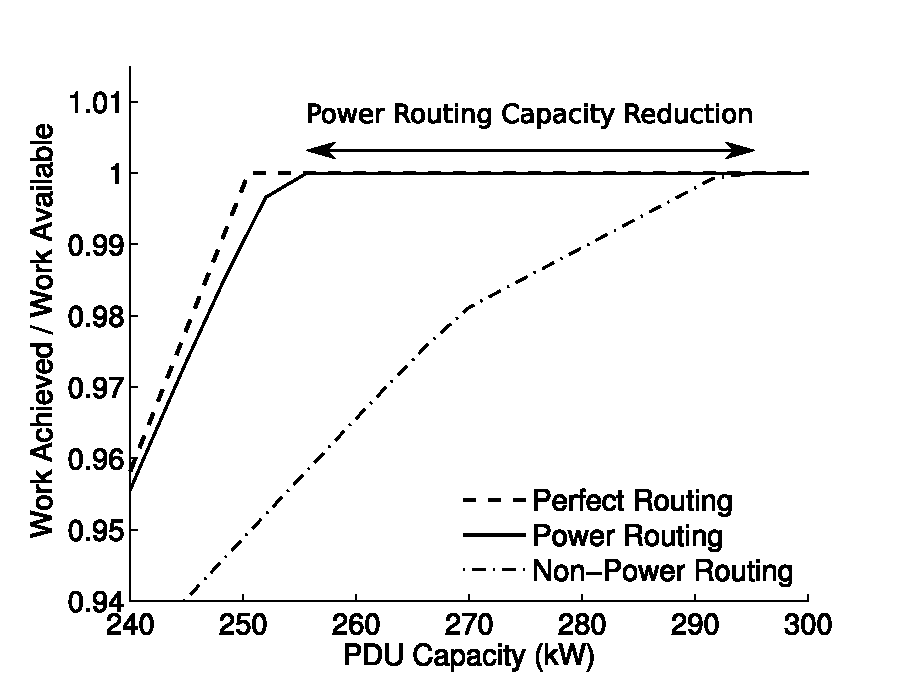
\includegraphics[width = 3.0 in]{Appendices/PowerRouting/figure/RoutingComparison.eps}
\caption{ \textbf{Shuffled Topologies: 6 PDUs, fully-connected}}
\label{figure::routingdemonstration}
\vspace{-.1 in}
\end{figure}

\subsection{Operating Principle.}

\PowerRouting relies on the observation that individual PDUs are unlikely to reach peak load simultaneously.
The power distribution system as a whole operates in one of three regimes.
The first, most common case is that the load on all PDUs is below their capacity.  In this case, the power infrastructure is over-provisioned, power capping is unnecessary, and the entire data center operates at full performance. At the opposite extreme, when servers demand more power than is available, the power infrastructure is under-provisioned, all PDUs will be fully loaded, and power capping (e.g., via performance throttling) is necessary.  In either of these regimes, \PowerRouting has no impact; the power infrastructure is simply under- (over-) provisioned relative to the server demand. 

\PowerRouting is effective in the intermediate regime where some PDUs are overloaded while others have spare capacity.  In current data centers, this situation will result in performance throttling that \PowerRouting can avoid.

To illustrate how \PowerRouting affects performance throttling, we explore its performance envelope near the operating region where aggregate power infrastructure capacity precisely meets demand.  Figure~\ref{figure::routingdemonstration} shows the relationship between installed PDU capacity and performance throttling (in terms of the fraction of offered load that is met) with and without  \PowerRouting (6 PDUs, fully-connected topology) and contrast these against an ideal, perfectly-balanced power distribution infrastructure.    The ideal infrastructure can route power from any PDU to any server and can split load fractionally over multiple PDUs.  (We detail the methodology used to evaluate \PowerRouting and produce these results in Section~\ref{section::methodology} below.)

The graph provides two insights into the impact of \PowerRouting.  First, we can use it to determine how much more performance \PowerRouting achieves for a given infrastructure investment relative to conventional and ideal designs.  This result can be obtained by comparing vertically across the three lines for a selected PDU capacity. As can be seen, \PowerRouting closely tracks the performance of the ideal power delivery infrastructure, recovering several percent of lost performance relative to a fully-connected topology without power routing.

The graph can also be used to determine the capital infrastructure savings that \PowerRouting enables while avoiding performance throttling altogether.  Performance throttling becomes necessary at the PDU capacity where each of the three power distributions dips below 1.0.  The horizontal distance between these intercepts is the capacity savings, and is labeled  ``Power Routing Capacity Reduction" in the figure. In the case shown here, \PowerRouting avoids throttling at a capacity of 255 kW, while 294 kW of capacity are needed without \PowerRouting. \PowerRouting avoids throttling, allowing maximum performance with less investment in power infrastructure.


% Scheduling
\section{Scheduling}
\label{section::scheduling}

\PowerRouting relies on a centralized scheduling algorithm to assign power to servers. Each time a server requests additional power (as a result of exhausting its power cap) the scheduler checks if the server's current active power feed has any remaining capacity, granting it if possible. If no slack exists, the scheduler attempts to create a new allocation schedule for the entire facility that will eliminate or minimize the need for capping. In addition to considering the actual desired power budget of each server, the scheduler must also provision sufficient reserve capacity on each feed such that the feed can sustain its share of load if any PDU fails.  Finally, we constrain the scheduler to allow only phase-balanced assignments where the load on the three phases of any PDU differ by no more than 20\% of the per-phase capacity.

The scheduling process comprises three steps: gathering the desired budget for each server, solving for an assignment of servers to their primary or secondary feeds, and then, if necessary, reducing server's budgets to meet the capacity constraints on each feed.

Whereas sophisticated methods for predicting power budgets are possible \cite{Choi08}, we use a simple policy of assigning each server a budget based on its average power demand in the preceding minute.  More sophisticated mechanisms are orthogonal to the scheduling problem itself.

Solving the power feed assignment problem optimally, even without redundancy, is an NP-Complete problem.  It is easy to see that power scheduling $\in$ NP; a nondeterministic algorithm can enumerate a set of assignments from servers to PDUs and then check in polynomial time that each PDU is within its power bounds.  To show that power scheduling is NP-Complete we transform PARTITION to it \cite{GareyBook}.  For a given instance of PARTITION of finite set $A$ and a size $s(a) \in \field{Z+}$ for each $a \in A$: we would like to determine if there is a subset $A' \in A$ such that the $\sum_{a \in A'}{s(a)} = \sum_{a \in A-A'}{s(a)}$. Consider $A$ as the set of servers, with $s(a)$ corresponding to server power draw. Additionally consider two PDUs each of power capacity $\sum_{a} s(a) / 2$. These two problems are equivalent. Thus, a polynomial time solution to power scheduling will yield a polynomial time solution to PARTITION (implying power scheduling is NP-Complete).

In data centers of even modest size, brute force search for an optimal power feed assignment is infeasible.  Hence, we resort to a heuristic approach to generate an approximate solution.  

We first optimally solve a power feed assignment problem allowing servers to be assigned fractionally across feeds using linear programming.  This linear program can be solved in polynomial time using standard methods \cite{CormenBook}. From the exact fractional solution, we then construct an approximate solution to the original problem (where entire servers must be assigned a power feed).  Finally, we check if the resulting assignments are below the capacity of each power feed.  If any feed's capacity is violated, we invoke a second optimization step to choose power caps for all servers.  

Determining optimal caps is non-trivial because of the interaction between a server's power allocation on its primary feed, and the reserve capacity that allocation implies on its secondary feed.  We employ a second linear programming step to determine a capping strategy that maximizes the amount of power allocated to servers (as opposed to reserve capacity).

{\bf Problem formulation.} We formulate the linear program based on the power distribution topology (i.e., the static assignment of primary and secondary feeds to each server), the desired server power budgets, and the power feed capacities.  For each pair of power feeds we calculate $Power_{i,j}$, the sum of power draws for all servers connected to feeds $i$ and $j$. (Our algorithm operates at the granularity of individual phases of AC power from each PDU, as each phase has limited ampacity). $Power_{i,j}$ is 0 if no server shares feeds  $i$ and $j$ (e.g., if the two feeds are different phases from the same PDU or no server shares those PDUs).  Next, for each pair of feeds, we define variables $Feed_{i,j}i$ and $Feed_{i,j}j$ to account for the server power from $Power_{i,j}$ routed to feeds $i$ and $j$, respectively.  Finally, a single global variable, $Slack$, represents the maximum unallocated power on any phase after all assignments are made.  
With these definitions, the linear program maximizes $Slack$ subject to the following constraints:

$\forall i, j \neq i$, $i$ and $j$ are any phases on different PDUs:

\vspace{-.2 in}
\begin{equation}\label{rationalbin}
Feed_{i,j}i + Feed_{i,j}j = Power_{i,j}
\end{equation}

\vspace{-.25 in}
\begin{equation}\label{pducapacity}
\displaystyle\sum_{k \neq i} Feed_{i,k}i + \displaystyle\sum_{l in j's PDU} Feed_{i,l}l + Slack \le Capacity(i) 
\end{equation}
\vspace{-.15 in}

And constraints for distinct phases $i$ and $j$ within a single PDU:

\vspace{-.2 in}
\begin{equation}\label{phasebalance}
|\displaystyle\sum_{k \neq i} Feed_{i,k}i - \displaystyle\sum_{k \neq j} Feed_{j,k}j| \le .2 \times Capacity(i,j)
\end{equation}
\vspace{-.15 in}

With the following bounds:

\vspace{-.2 in}
\begin{equation}\label{freeslack}
-\infty \le Slack \le \infty
\end{equation}
\vspace{-.15 in}

\vspace{-.25 in}
\begin{equation}\label{positivefeeds}
\forall i, j \ne i : Feed_{i,j}i, Feed_{i,j}j \ge 0
\end{equation}
\vspace{-.15 in}

Equation \ref{rationalbin} ensures that power from servers connected to feeds $i$ and $j$ is assigned to one of those two feeds.
Equation \ref{pducapacity} restricts the sum of all power assigned to a particular feed $i$, plus the reserve capacity required on $i$ should feeds on  $j$'s PDU fail, plus the excess slack to be less than the capacity of feed $i$. Finally, equation \ref{phasebalance} ensures that phases are balanced across each PDU. A negative $Slack$ indicates that more power is requested by servers than is available (implying that there is no solution to the original, discrete scheduling problem without power capping).

We use the fractional power assignments from the linear program to schedule servers to feeds.
For a given set of servers, $s$, connected to both feed $i$ and feed $j$, the fractional solution will indicate that $Feed_{i,j}i$ watts be assigned to $i$ and $Feed_{i,j}j$ to $j$.  The scheduler must create a discrete assignment of servers to feeds to approximate the desired fractional assignments as closely as possible, which is itself a bin packing problem.  To solve this sub-problem efficiently, the scheduler sorts the set $s$ descending by power and repeatedly assign the largest unassigned server to $i$ or $j$, whichever has had less power assigned to it thus far (or whichever has had less power relative to its capacity if the capacities differ).

If a server cannot be assigned to either feed without violating the feed's capacity constraint, then throttling may be necessary to achieve a valid schedule.  The server is marked as ``pending" and left temporarily unassigned. By the nature of the fractional solution, at most one server in the set can remain pending.  This server must eventually be assigned to one of the two feeds; the difference between this discrete assignment and the optimal fractional assignment is the source of error in our heuristic. By assigning the largest servers first we attempt to minimize this error. Pending servers will be assigned to the feed with the most remaining capacity once all other servers have been assigned.

The above optimization algorithm assumes that each pair of power feeds shares several servers in common, and that the power drawn by each server is much less than the capacity of the feed.
We believe that plausible power distribution topologies fit this restriction.

Following server assignment, if no feed capacity constraints have been violated, the solution is complete and all servers are assigned caps at their requested budgets.  If any slack remains on a feed, it can be granted upon a future request without re-invoking the scheduling mechanism, avoiding unnecessary switching. 

If any capacity constraints have been violated, a new linear programming problem is formulated to select power caps that maximize the amount of power allocated to servers (as opposed to reserve capacity for fail-over).  We scale back each feed such that no PDU supplies more power than its capacity, even in the event that another PDU fails.  The objective function maximizes the sum of the server budgets.  We assume that servers can be throttled to any frequency from idle to peak utilization and that the relationship and limits of frequency and power scaling are known a priori.
Note, however, that this formulation ignores heterogeneity in power efficiency, performance, or priority across servers; it considers only the redundancy and topology constraints of the power distribution network.  An analysis of more sophisticated mechanisms for choosing how to cap servers that factors in these considerations is outside the scope of this paper.



% Evaluation
\section{Evaluation}
\label{section::evaluation}

Our evaluation demonstrates the effectiveness of shuffled topologies and \PowerRouting at reducing the required capital investment in power infrastructure to meet a high-availability data center's reliability and power needs.  First, we demonstrate how shuffled topologies reduce the reserve capacity required to provide single-PDU-fault tolerance.  Then, we examine the effectiveness of \PowerRouting at further reducing provisioning requirements as a function of topology, number of PDUs, and workload.  Finally, we show how \PowerRouting will increase in effectiveness as server power management becomes more sophisticated and the gap between servers' idle and peak power demands grows.

\subsection{Methodology}
\label{section::methodology}

We evaluate \PowerRouting through analysis of utilization traces from a large collection of production systems. We simulate \PowerRouting's scheduling algorithm and impact on performance throttling and capital cost.

{\bf Traces.}
We collect utilization traces from three production facilities: (1) \emph{EECS servers}, a small cluster of departmental servers (web, email, login, etc.) operated by the Michigan EECS IT staff; (2) \emph{Arbor Lakes Data Center}, a ~1.5MW facility supporting the clinical operations of the University of Michigan Medical Center; and (3) \emph{Michigan Academic Computer Center (MACC)}, a 4MW high-performance computing facility operated jointly by the University of Michigan, Internet2, and Merit that runs primarily batch processing jobs.  These sources provide a diverse mix of real-world utilization behavior.  Each of the traces ranges in length from three to forty days sampling server utilization once per minute.  We use these traces to construct a hypothetical high-availability hosting facility  comprising 400 medical center servers, 300 high performance computing nodes, and a 300-node web search cluster.   The simulated medical center and HPC cluster nodes each replay a trace from a specific machine in the corresponding real-world facility.  The medical center systems tend to be lightly loaded, with one daily utilization spike (which we believe to be daily backup processing).  The HPC systems are heavily loaded.  As we do not have access to an actual 300-node web search cluster, we construct a cluster by replicating the utilization trace of a single production web server over 300 machines.  The key property of this synthetic search cluster is that the utilization on individual machines rises and falls together in response to user traffic, mimicking the behavior reported for actual search clusters \cite{Fan07}.  We analyze traces for a 24-hour period. Our synthetic cluster sees a time-average power draw of 180.5 kW, with a maximum of 208.7 kW and standard deviation of 9 kW.

{\bf Power.}  We convert utilization traces to power budget requests using published SPECPower results \cite{SpecPower}.  Most of our traces have been collected from systems where no SPECPower result has been published; for these, we attempt to find the closest match based on vendor descriptions and the number and model of CPUs and installed memory. As SPECPower only provides power at intervals of 10\% utilization, we use linear interpolation to approximate power draw in between these points.

Prior work \cite{Fan07,Ranganathan06} has established that minute-grained CPU utilization traces can predict server-grain power 
draw to within a few percent.   Because of the scope of our data collection efforts, finer-grained data collection is impractical.  Our estimates of savings from Power Routing are conservative; finer-grained scheduling might allow tighter tracking of instantaneous demand.  

To test our simulation approach, we have validated simulation-derived power values against measurements of individual servers in our lab.    Unfortunately, the utilization and power traces available from our production facilities are not exhaustive, which precludes a validation experiment where we compare simulation-derived results to measurements for an entire data center.
 
{\bf Generating data center topologies.} For each power distribution topology described in Section~\ref{section::intermixed}, we design a layout of our hypothetical facility to mimic the typical practices seen in the actual facilities. We design layouts according to the policies the Michigan Medical Center IT staff use to manage their \emph{Arbor Lakes} facility. Each layout determines an assignment of physical connections from PDUs to servers. Servers that execute similar applications are collocated in the same rack, and, hence, in conventional power delivery topologies, are connected to the same PDU.  Where available, we use information about the actual placement of servers in racks to guide our placement.  Within a rack, servers are assigned across PDU phases in a round-robin fashion.  We attempt to balance racks across PDUs and servers within racks across AC phases based on the corresponding system's power draw at 100\% utilization.  No server is connected to two phases of the same PDU, as this arrangement does not protect against PDU failure.  We use six PDUs in all topologies unless otherwise noted.

{\bf Metrics.} We evaluate \PowerRouting based on its impact on server throttling activity and data center capital costs.  As the effect of voltage and frequency scaling on performance varies by application, we instead use the fraction of requested server power budget that was not satisfied as a measure of the performance of capping techniques.  Under this metric, the ``cost" of failing to supply a watt of requested power is uniform over all servers, obviating the need to evaluate complex performance-aware throttling mechanisms (which are orthogonal to \PowerRouting). Our primary evaluation metric is the minimum total power delivery capacity required to assure zero performance throttling, as this best illustrates the advantage of \PowerRouting over conventional worst-case provisioning.

\subsection{Impact of Shuffled Topologies}

\begin{figure}[t!]
\centering
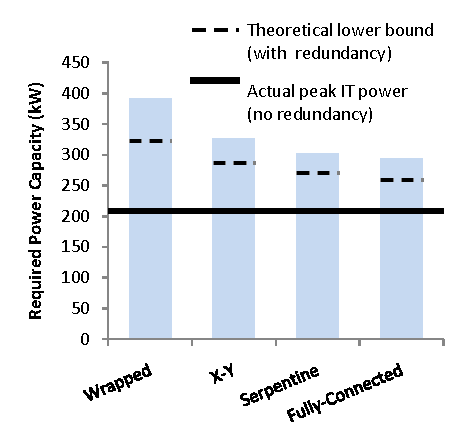
\includegraphics[width = 3.0 in]{Appendices/PowerRouting/figure/result_intermix.eps}
\caption{ \textbf{Minimum capacity for redundant operation under shuffled topologies (no Power Routing).} }
\label{figure::intermix}
\vspace{-.1 in}
\end{figure}

We first compare the impact of shuffled topologies on required power infrastructure capacity.  Shuffled topologies reduce the reserve capacity that each PDU must sustain to provide fault tolerance against single-PDU failure.  We examine the advantage of several topologies relative to the baseline high-availability ``wrapped" data center topology, which requires each PDU to be over-provisioned by 50\% of its nominal load.  We report the total power capacity required to prevent throttling for our traces.  We assume that each PDU must maintain sufficient reserve capacity at all times to precisely support the time-varying load that might fail over to it.

Differences in the connectivity of the various topologies result in differing reserve capacity requirements.
For an ideal power distribution infrastructure (one in which load is perfectly balanced across all PDUs), each PDU must reserve $\frac{1}{c + 1}$ to support its share of a failing PDU's load, where $c$ is the \emph{fail-over connectivity} of the PDU.  Fail-over connectivity counts the number of distinct neighbors to which a PDU's servers will switch in the event of failure. It is two for the wrapped topology, four for serpentine, and varies as a function of the number of PDUs for X-Y and fully-connected topologies. As the connectivity increases, reserve requirements decrease, but with diminishing returns.

To quantify the impact of shuffled topologies, we design an experiment where we statically assign each server the best possible primary and secondary power feed under the constraints of the topology.  We balance the average power draw on each PDU using each server's average power requirement over the course of the trace. (We assume this average to be known a priori for each server.)  

In Figure~\ref{figure::intermix} each bar indicates the required power capacity for each topology to meet its load and reserve requirements in all time epochs  (i.e., no performance throttling or loss of redundancy) for a 6 PDU data center.  For 6 PDUs, the fail-over connectivities are 2, 3, 4, and 5 for the wrapped, X-Y, serpentine, and fully-connected topologies, respectively.  The dashed line on each bar indicates the topology's theoretical lower-bound capacity requirement to maintain redundancy if server power draw could be split dynamically and fractionally across primary and secondary PDUs (which \PowerRouting approximates).  The gap between the top of each bar and the dashed line arises because of the time-varying load on each server, which creates imbalance across PDUs and forces over-provisioning. The solid line crossing all bars indicates the data center's peak power draw, ignoring redundancy requirements (i.e., the actual peak power supplied to IT equipment).

Topologies with higher connectivity require less reserve capacity, though the savings taper off rapidly.  The X-Y and serpentine topologies yield impressive savings and are viable and scalable from an implementation perspective.  Nevertheless, there is a significant gap between the theoretical (dashed) and practical (bar) effectiveness of shuffled topologies.  As we show next, \PowerRouting closes this gap.   

\subsection{Impact of \PowerRouting}
\label{sec::routing}

{\bf \PowerRouting effectiveness.}
To fully explore \PowerRouting effectiveness, we repeated the analysis above for all four topologies (wrapped, X-Y, serpentine, and fully-connected) and contrast the capacity required to avoid throttling for each. For comparison, we also reproduce the capacity requirements without \PowerRouting (from Figure~\ref{figure::intermix}).  We show results in Figure~\ref{figure::powerrouting}.
Again, a dashed line represents the theoretical minimum capacity necessary to maintain single-PDU fault redundancy for our workload and the given topology; the solid line marks the actual peak IT power draw. Because the overall load variation in our facilities is relatively small (HPC workloads remain pegged at near-peak utilization; the medical facility is over-provisioned to avoid overloading), we expect a limited opportunity for \PowerRouting.  Nonetheless, we reduce required power delivery capacity for all topologies (except wrapped) by an average of 12\%.

From the figure, we see that the sparsely-connected wrapped topology is too constrained for \PowerRouting to be effective; \PowerRouting requires 20\% more than the theoretical lower bound infrastructure under this topology. The three shuffled topologies, however, nearly reach their theoretical potential, even with a heuristic scheduling algorithm.
Under the fully-connected topology, \PowerRouting comes within 2\% of the bound, reducing power infrastructure requirements by over 39kW (13\%) relative to the same topology without \PowerRouting and more than 35\% relative to the baseline wrapped topology without \PowerRouting.
Our result indicates that more-connected topologies offer an advantage to \PowerRouting by providing more freedom to route power.
However, the the more-practical topologies yield similar infrastructure savings; the serpentine topology achieves 32\% savings relative to the baseline.

\begin{figure}[t!]
\centering
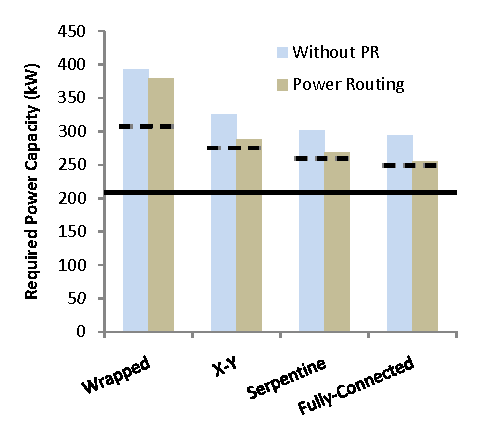
\includegraphics[width = 3.0 in]{Appendices/PowerRouting/figure/result_powerrouting.eps}
\caption{ \textbf{\PowerRouting infrastructure savings as a function of topology.} }
\label{figure::powerrouting}
\vspace{-.1 in}
\end{figure}

{\bf Sensitivity to number of PDUs.}
The number of PDUs affects \PowerRouting effectiveness, particularly for the fully-connected topology. Figure~\ref{figure::pdus} shows this sensitivity for four to eight PDUs. For a fixed total power demand, as the number of PDUs increases, each individual PDU powers fewer servers and requires less capacity.  With fewer servers, the variance in power demands seen by each PDU grows (i.e., statistical averaging over the servers is lessened), and it becomes more likely that an individual PDU will overload. Without \PowerRouting, this effect dominates, and we see an increase in required infrastructure capacity as the number of PDUs increases beyond 6.  At the same time, increasing the number of PDUs offers greater connectivity for certain topologies, which in turn lowers the required slack that PDUs must reserve and offers \PowerRouting more choices as to where to route power.  Hence, \PowerRouting is better able to track the theoretical bound and the required power capacity decreases with more PDUs.


\begin{figure}[t!]
\centering
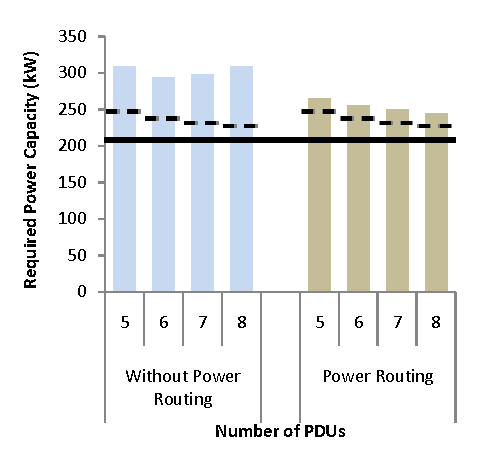
\includegraphics[width = 3.0 in]{Appendices/PowerRouting/figure/result_numPDUs.eps}
\caption{ \textbf{Sensitivity of the fully-connected topology to number of PDUs.} }
\label{figure::pdus}
\vspace{-.1 in}
\end{figure}

\subsection{\PowerRouting For Low Variance Workloads}
%{\bf \PowerRouting for low variance workloads.}
The mixed data center trace we study is representative of the diversity typical in most data centers.  Nevertheless, some data centers run only a single workload on a homogeneous cluster.  \PowerRouting exploits diversity in utilization patterns to shift power delivery slack; hence, its effectiveness is lower in homogeneous clusters.  

\begin{figure*}[t]
\centering
\subfigure[Arbor Lakes (clinical operations)]{
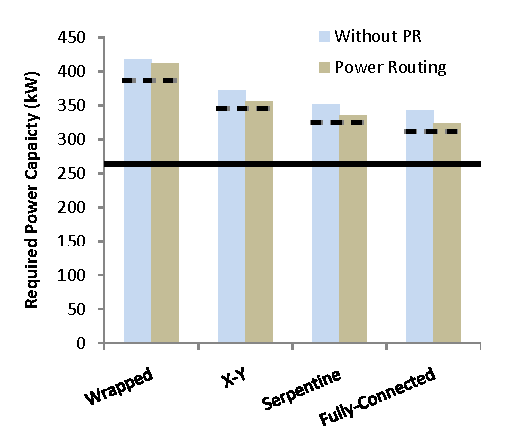
\includegraphics[width=3.0 in]{Appendices/PowerRouting/figure/result_AL.eps}
\label{figure::AL}
}
\hspace{0.5in}
\subfigure[MACC (high-performance computing)]{
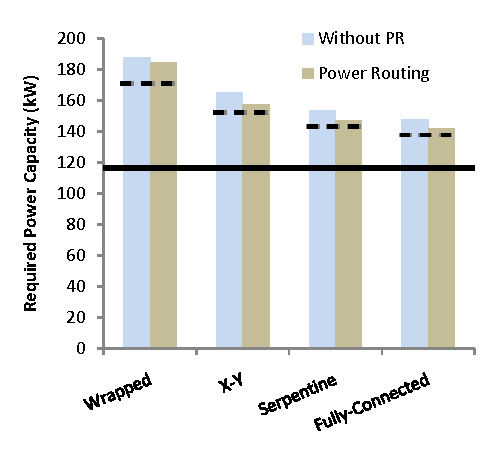
\includegraphics[width=3.0 in]{Appendices/PowerRouting/figure/result_nyx.eps}
\label{figure::nyx}
}
\vspace{-0.15 in}
\caption{ \textbf{\PowerRouting effectiveness in homogeneous data centers.} }
\vspace{-0.15 in}
\label{figure::homogenous}
\end{figure*}

To explore these effects, we construct \PowerRouting test cases for 1000-server synthetic clusters where each server runs the same application.  We do not study the web search application in isolation; in this application, the utilization on all servers rise and fall together, hence, the load on all PDUs is inherently balanced and there is no opportunity (nor need) for \PowerRouting. Instead, we evaluate \PowerRouting using the medical center traces and high performance computing traces, shown in Figures~\ref{figure::AL} and \ref{figure::nyx}, respectively. 

The high performance computing cluster consumes a time-average power of 114.9 kW, a maximum of 116.4 kW, and a standard deviation of 0.8 kW while the medical center computing traces consume a time-average power of 254.6 kW, with maximum 263.6 kW and standard deviation 2.4 kW.  In both cases, the variability is substantially lower than in the heterogeneous data center test case.

Although \PowerRouting comes close to achieving the theoretical lower bound infrastructure requirement in each case, we see that there is only limited room to improve upon the non-\PowerRouting case. Even the baseline wrapped topology requires infrastructure that exceeds the theoretical bound by only 7.5\% for the high performance computing cluster and 5\% for the medical data center. We conclude that \PowerRouting offers substantial improvement only in heterogeneous clusters and applications that see power imbalance, a common case in many facilities.

\subsection{\PowerRouting With Energy-Proportional Servers}
%{\bf \PowerRouting with Energy-Proportional Servers.}
As the gap between servers' peak and idle power demands grows  (e.g., with the advent of energy-proportional computers \cite{Barroso07}), we expect the potential for \PowerRouting to grow. The increase in power variance leads to a greater imbalance in power across PDUs, increasing the importance of correcting this imbalance with \PowerRouting.

To evaluate this future opportunity, we perform an experiment where we assume all servers are energy-proportional---that is, servers whose power draw varies linearly with utilization---with an idle power of just 10\% of peak.  This experiment models servers equipped with PowerNap \cite{Meisner09}, which allows servers to sleep during the millisecond-scale idle periods between task arrivals.  We repeat the experiment shown in Figure~\ref{figure::powerrouting} under this revised server power model. The results are shown in Figure~\ref{figure::powernap}.  Under these assumptions, our traces exhibit a time-average power of 99.8 kW, maximum of 153.9 kW, and standard deviation of 18.9 kW.

\PowerRouting is substantially more effective when applied to energy-proportional servers. 
However, the limitations of the wrapped topology are even more pronounced in this case, and \PowerRouting provides little improvement. Under the more-connected topologies, \PowerRouting is highly effective, yielding reductions of 22\%, 29\%, and 28\% for the X-Y, serpentine, and fully-connected topologies, respectively, relative to their counterparts without \PowerRouting.
As before, the more-connected topologies track their theoretical lower bounds more tightly.  Relative to the baseline wrapped topology, a serpentine topology with \PowerRouting yields a 47\% reduction in required physical infrastructure capacity. It is likely that as computers become more energy-proportional, power infrastructure utilization will continue to decline due to power imbalances.
\PowerRouting reclaims much of this wasted capacity.

\begin{figure}[t!]
\centering
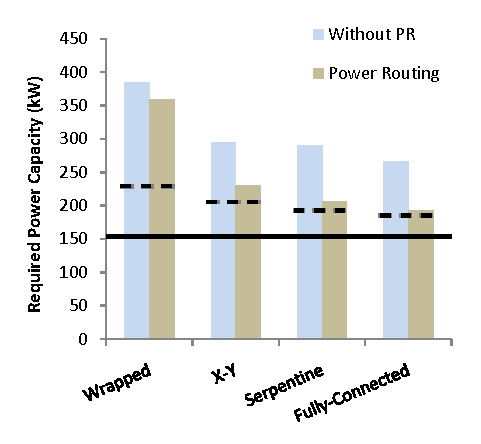
\includegraphics[width = 3.0 in]{Appendices/PowerRouting/figure/result_powernap.eps}
\vspace{-.1 in}
\caption{ \textbf{Impact with energy-proportional servers.} }
\label{figure::powernap}
\vspace{-.15 in}
\end{figure}


\subsection{Limitations}

Our evaluation considers workloads in which any server may be throttled, and our mechanisms make no effort to select servers for throttling based on any factors except maximizing the utilization of the power delivery infrastructure.  In some data centers, it may be unacceptable to throttle performance.  These data centers cannot gain a capital cost savings from under-provisioning; their power infrastructure must be provisioned for worst case load.  Nonetheless, these facilities can benefit from intermixed topologies (to reduce reserve capacity for fault tolerance) and from the phase-balancing possible with \PowerRouting.
 

% Conclusion
\section{Conclusion}
\label{section::conclusion}

The capital cost of power delivery infrastructure is one of the largest components of data center cost, rivaling energy costs over the life of the facility.  In many data centers, expansion is limited because available power capacity is exhausted.  To extract the most value out of their infrastructure, data center operators over-subscribe the power delivery system.  As long as individual servers connected to the same PDU do not reach peak utilization simultaneously, over-subscribing is effective in improving power infrastructure utilization.  However, coordinated utilization spikes do occur, particularly among collocated machines, which can lead to substantial throttling even when the data center as a whole has spare capacity.

In this paper, we introduced a pair of complementary mechanisms, shuffled power distribution topologies and \PowerRouting, that reduce performance throttling and allow cheaper capital infrastructure to achieve the same performance levels as current data center designs.  Shuffled topologies permute power feeds to create strongly-connected topologies that reduce reserve capacity requirements by spreading responsibility for fault tolerance.  \PowerRouting schedules loads across redundant power delivery paths to shift power delivery slack to satisfy localized utilization spikes.  Together, these mechanisms reduce capital costs by 32\% relative to a baseline high-availability design when provisioning for zero performance throttling. Furthermore, with energy-proportional servers, the power capacity reduction increases to 47\%.


% Acknowledgements
%%%%%%%%%%%%%%%%%%%%%%%%%%%%%%%%%%% 
%				Acknowledgements 
%%%%%%%%%%%%%%%%%%%%%%%%%%%%%%%%%% 
\section*{Acknowledgements} 

The authors would like to thank Joseph Kryza and the University of Michigan Medical Center IT staff for facilitating access to the Arbor Lakes data center, Andrew Caird and the staff at the Michigan Academic Computer Center for assistance in collecting the high performance computing cluster data, Laura Fink for assistance in collecting the departmental server utilization traces, and Vikram Adve and the anonymous reviewers for their feedback. This work was supported by an equipment grant from Intel, financial support from the Michigan Medical Center IT department, and NSF grant CCF-0811320.



%%%\begin{spacing}{1.0}
%%%\bibliographystyle{IEEEtranS}
%%%\bibliography{abbrev,PowerRouting}
%%%\end{spacing}
%%%
%%%
%%%\end{document}
